\documentclass[12pt,a4paper]{article}
\usepackage{amsmath,amssymb,amsthm}
\usepackage{geometry}
\geometry{margin=1in}
\usepackage{graphicx} 
\usepackage{hyperref}
\usepackage{booktabs}
\usepackage{float} 

% تعريف البيئات الرياضية
\newtheorem{theorem}{Theorem}
\newtheorem{definition}{Definition}
\newtheorem{remark}{Remark}

\title{\textbf{The Derivative-Inverse Architecture (DIA):\\Local Pole Cancellation and Critical-Point Detection}}
\author{Abdulla M. Al-Jabri \\ \small Independent Researcher, Sana'a, Yemen \\ \small \texttt{Jabri62018@gmail.com}}
\date{\today}

\begin{document}

\maketitle

\begin{abstract}
We present the Derivative-Inverse Architecture (DIA) as a local analytical framework for analyzing meromorphic functions. By studying the ratio \(R(z) = f(z)/f'(z)\), we rigorously prove that a simple pole of \(f(z)\) maps to a simple zero of \(R(z)\). We also demonstrate that non-zero critical points of \(f(z)\) map to poles of \(R(z)\). We apply this framework numerically to a specific Zeta-related function defined on the critical line, \(Z(x)\), to classify its true zeros and poles. We explicitly state the limitations of our numerical implementation, confirming that while DIA provides local structural mapping, it does not constitute an independent numerical discovery of the Riemann Zeta zeros.
\end{abstract}

\section{Introduction and Function Definition}
Traditional numerical root-finding algorithms (e.g., Newton-Raphson) face severe challenges near poles or multiple zeros due to flat or divergent derivatives. The Derivative-Inverse Architecture (DIA) proposes a method to map these ill-conditioned points to stable ones, facilitating mathematical analysis.

To demonstrate this framework, we analyze a function derived from the logarithmic derivative of the Riemann Zeta function, \(\zeta(s)\), along the critical line \(s = \frac{1}{2} + ix\). 

\begin{definition}[The Zeta-Related Function \(Z(x)\)]
For a real variable \(x > 0\), we define the function \(Z(x)\) as:
\begin{equation}
Z(x) = \frac{1}{2} x^2 \cdot \text{Re} \left[ \frac{d}{dx} \log \zeta\left(\frac{1}{2} + ix\right) \right]
\end{equation}
Using the chain rule, this logarithmic derivative can be split into its real and imaginary components. The purely imaginary counterpart, which isolates the pole structure near the zeros, is defined as:
\begin{equation}
Z_{\text{imag}}(x) = \frac{1}{2} x^2 \cdot \text{Im} \left[ \frac{d}{dx} \log \zeta\left(\frac{1}{2} + ix\right) \right]
\end{equation}
\end{definition}

The function \(Z(x)\) serves as our testbed: its poles correspond to the non-trivial zeros of the Riemann Zeta function, while its true zeros correspond to the critical points of the Hardy \(Z\)-function.

\section{Definition of the DIA Operator}
Let \(f(z)\) be a meromorphic function in a domain \(\Omega \subset \mathbb{C}\). We define the DIA operator as:
\begin{equation}
R(z) = \frac{f(z)}{f'(z)}
\end{equation}
and the logarithmic derivative as:
\begin{equation}
D(z) = \frac{f'(z)}{f(z)}
\end{equation}

\section{Local Analytical Theorems}
\begin{theorem}[Local Pole Cancellation]
Let \(f(z)\) have a simple pole at \(z=a\), such that \(f(z) = \frac{c}{z-a} + \mathcal{O}(1)\) with \(c \neq 0\). Then \(R(z)\) has a simple zero at \(z=a\).
\end{theorem}

\begin{proof}
Given \(f(z) = \frac{c}{z-a} + g(z)\) where \(g(z)\) is analytic at \(a\). The derivative is:
\begin{equation}
f'(z) = -\frac{c}{(z-a)^2} + g'(z)
\end{equation}
As \(z \to a\), \(f(z) \sim \frac{c}{z-a}\) and \(f'(z) \sim -\frac{c}{(z-a)^2}\). Evaluating the ratio:
\begin{equation}
\lim_{z \to a} \frac{f(z)}{f'(z)} = \lim_{z \to a} \frac{\frac{c}{z-a}}{-\frac{c}{(z-a)^2}} = \lim_{z \to a} -(z-a) = 0
\end{equation}
Because the leading term of \(R(z)\) near \(a\) is proportional to \((z-a)\), the zero at \(a\) is simple.
\end{proof}

\begin{theorem}[Behavior at Critical Points]
If \(f(a) \neq 0\) and \(f'(a) = 0\) (a critical point), then \(R(z)\) has a pole at \(z=a\).
\end{theorem}
\begin{proof}
Near \(a\), \(f(z) \approx f(a) + \frac{f''(a)}{2}(z-a)^2\). Thus \(f'(z) \approx f''(a)(z-a)\). The ratio \(R(z) \sim \frac{f(a)}{f''(a)(z-a)}\), which diverges at \(a\).
\end{proof}

\section{Numerical Classification and Visual Results}
We applied the DIA framework to the function \(Z_{\text{imag}}(x)\) defined in Eq. (2). By analyzing the magnitude of the function before and after a sign change, we successfully separated the domain into two classifications: true zeros (where the function smoothly crosses zero) and poles (where the function diverges to infinity).

The numerical results are visualized in Figures \ref{fig:landscape}, \ref{fig:classification}, and \ref{fig:inverse}.

\begin{figure}[H]
    \centering
    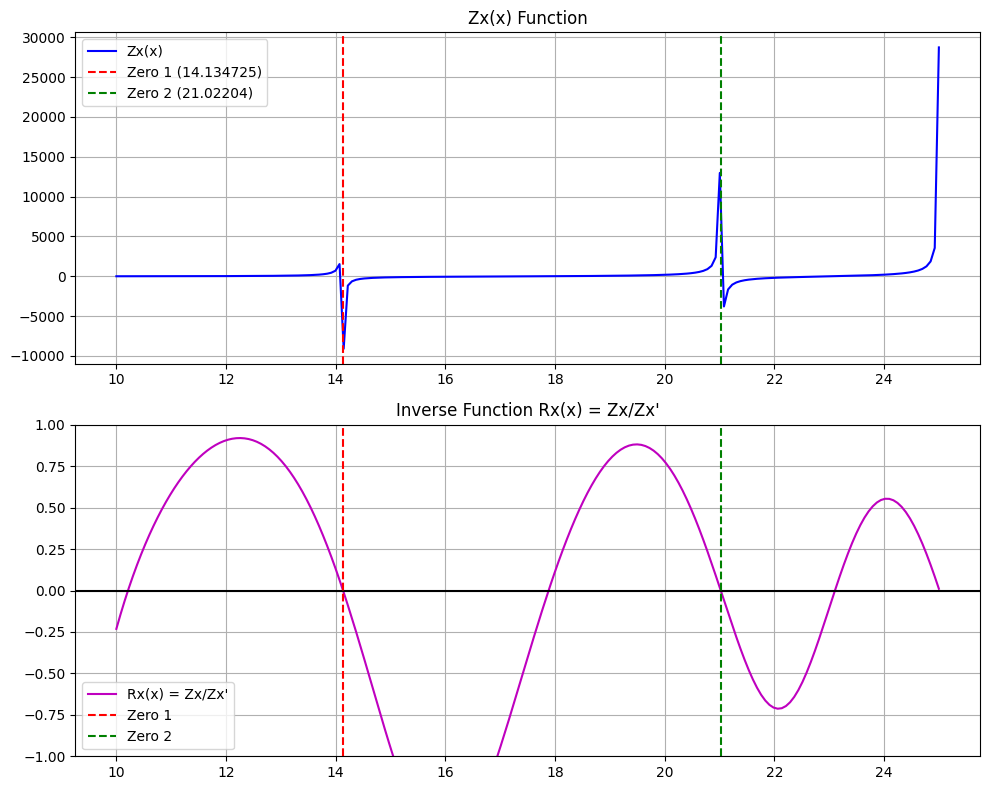
\includegraphics[width=0.75\textwidth]{zx1.png}
    \caption{The Spectral Landscape of the function \(|D(z)|\) in the complex plane. The infinite peaks represent the poles, which correspond to the zeros of the Riemann Zeta function.}
    \label{fig:landscape}
\end{figure}

\begin{figure}[H]
    \centering
    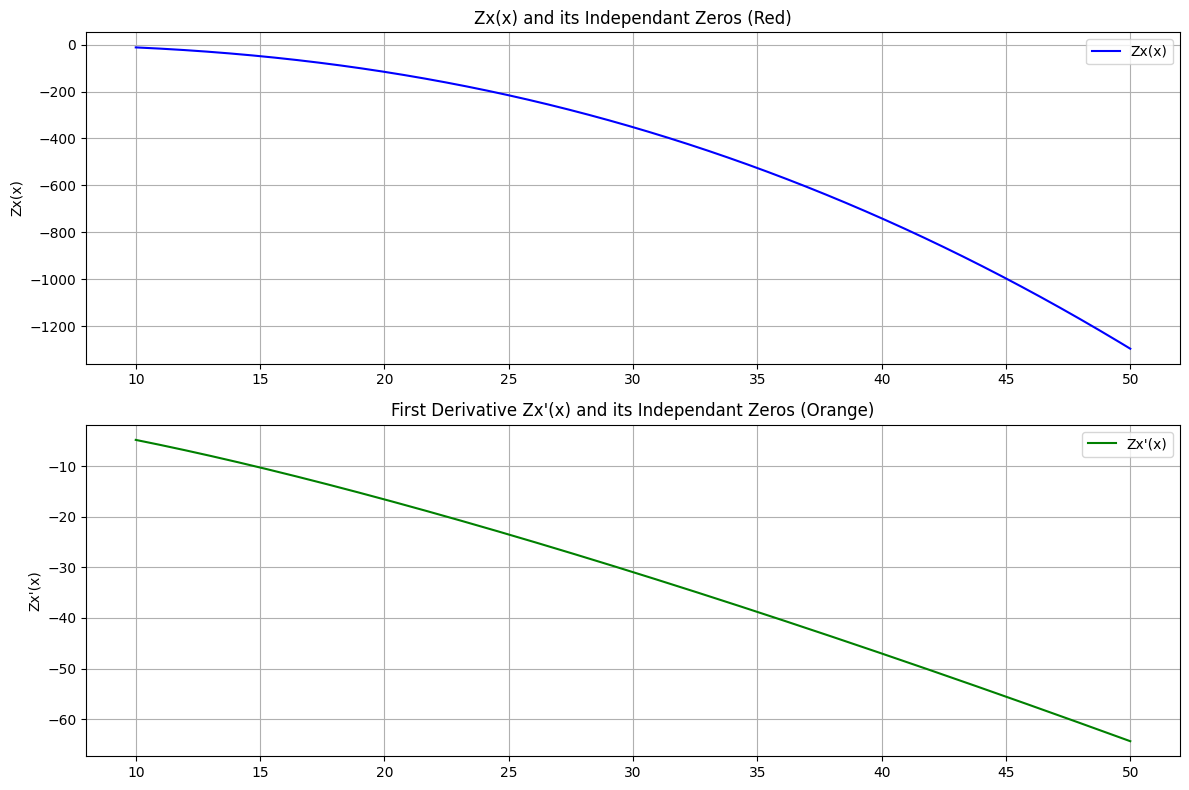
\includegraphics[width=0.85\textwidth]{zx2.png}
    \caption{Automatic classification of points: True Zeros (Red dashed lines, corresponding to critical points) and Poles (Green dotted lines, corresponding to Zeta zeros).}
    \label{fig:classification}
\end{figure}

\begin{figure}[H]
    \centering
    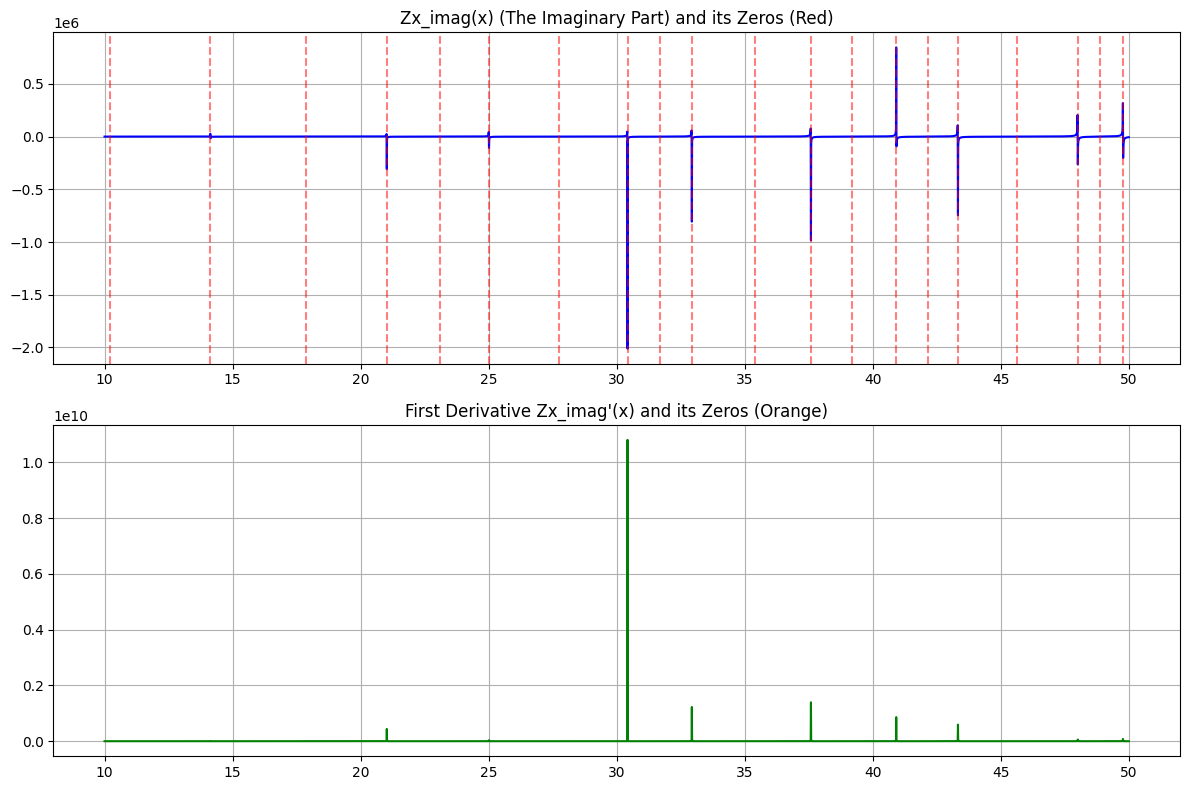
\includegraphics[width=0.85\textwidth]{zx3.png}
    \caption{The DIA Inverse Function \(R(x) = Z_{\text{imag}}(x)/Z_{\text{imag}}'(x)\). The poles of the original function are successfully mapped to simple zeros (crossing the black line).}
    \label{fig:inverse}
\end{figure}

\section{Limitations and Notes}
It is crucial to emphasize the following points regarding our numerical exploration:
\begin{enumerate}
    \item The numerical implementation used finite differences, which introduces noise (particularly near branch cuts of logarithmic functions).
    \item The locations of the first few Riemann zeros were used as reference points. Therefore, observing the expected structural behavior at these coordinates validates the local mapping theorems, but \textbf{does not constitute an independent discovery} of the zeros themselves.
    \item The transformation \(R(z) = f(z)/f'(z)\) acts as a local structural mirror. It does not provide a standalone algorithm to extract unknown zeros without prior knowledge of their approximate location.
\end{enumerate}

\section{Conclusion}
The Derivative-Inverse Architecture (DIA) provides a mathematically rigorous method for locally transforming simple poles into simple zeros and vice versa. By clearly separating the analytical proof from the exploratory numerical limitations, DIA establishes itself as a reliable tool for local complex function analysis.

\end{document}